\setcounter{chapter}{-1}
\chapter{Preface}
\section{$1^{st}$ Edition}
This book presents the results of Project Oberon, namely an entire software environment for a
modern workstation. The project was undertaken by the authors in 1986-89, and its
primary goal was to design and implement an entire system from scratch, and to structure it in
such a way that it can be described, explained, and understood as a whole. In order to become
confronted with all aspects, problems, design decisions and details, the authors not only
conceived but also programmed the entire system described in this book, and more.

Although there exist numerous books explaining principles and structures of OSes,
there is a lack of descriptions for one actually implemented and used. We wished not only to
give advice on how a system might be built, but to demonstrate how one was built. Program
listings therefore play a key role in this text, because they alone contain the ultimate explanations.
The choice of a suitable formalism therefore assumed great importance, and we designed the
language Oberon as not only an effective vehicle for implementation, but also as a publication
medium for algorithms in the spirit in which Algol 60 had been created three decades ago.
Because of its structure, the language Oberon is equally well suited to exhibit global, modular
structures of programmed systems.

In spite of the small number of man-years spent on realizing the Oberon, and in spite of its
compactness letting whose description fit a single book, it is not an academic toy, but rather a versatile
workstation system that has found many satisfied and even enthusiastic users in academia and
industry. The core system described here, consisting of storage, file, display, text, and viewer
managers, of program loader and device drivers, draws its major power from a suitably chosen,
flexible set of basic facilities and, most importantly, of their effective extensibility in many
directions and for many applications. The latter is particularly enhanced by the language
Oberon on the one, and by the efficiency of its basic core on the other hand. It is rooted in the
application of the object-oriented paradigm which is employed wherever extensibility appears advantageous.

In addition to the core system, we describe in full detail the compiler for language Oberon and
a graphics system, which both may be regarded as applications. The former reveals how a
compact compiler is designed to achieve both fast compilation and efficient, dense code. The
latter stands as an example of extensible design based on object-oriented techniques, and it
shows how a proper integration with an existing text system is possible. A network module is 
another addition to the core system allowing many workstations to be interconnected. We also show
how the Oberon serves conveniently as the basis for a multi-server station,
accommodating a file distribution, a printing, and an electronic-mail facility.

Compactness and regular structure, and due attention to efficient implementation of important
details appear to be the key to economical software engineering. With the Oberon, we
wish to refute Reiser's Law, which has been confirmed by virtually all recent releases of operating
systems: In spite of great leaps forward, hardware being becoming faster is more slowly than software 
being slower. The Oberon has required a tiny fraction of the manpower demanded for
the construction of widely-used commercial OSes, and a small fraction of their
demands on computing power and storage capacity, while providing equal power and flexibility to
the user, albeit without certain bells and whistles. The reader is invited to study how this was
possible.

But most importantly, we hope to present a worth-while case study of a substantial piece of
programming in large for the benefit of all those who are eager to learn from the experiences of others.

We wish to thank the many anonymous contributors of suggestions, advice, and encouragement.
In particular we wish to thank our colleagues H. Mössenböck, B. Sanders and our associates
at the Institut für Computer systeme for reading all or parts of the book draft. We are grateful
to M. Brandis, R. Crelier, A. Disteli, M. Franz, and J. Templ for their work in porting the Oberon
System successfully to various commercially available computers, and thus making the study of
this book more worth-while for many readers. And we gratefully acknowledge the contribution of
our school, ETH, for providing the environment and support which made it possible for us to
pursue and complete this project.
\begin{flushright}
  Zürich, February 1992 \\
  N.W. and J.G.
\end{flushright}

\clearpage\section{$2^{nd}$ Edition}
Comments about plans to prepare a second edition to this book varied widely. Some felt that this
book is outdated, that nobody is interested in a system of this kind any longer. "Why bother"?
Others felt that there is an urgent need for this type of text, which explains an entire system in detail
rather than merely proposing strategies and approaches. "By all means"!.

Very much has changed in these last 30 years. But even without this change, it would be
preposterous to propose and construct a system competing with existing, worldwide "standards".
Indeed, very few people would be interested in using it. The community at large seems to be stuck
with these gigantic software systems, and helpless against their complexity, peculiarities, and occasional unreliability.

But surely new systems will emerge, perhaps for different, limited purposes, allowing for smaller
systems. One wonders where their designers will study and learn their trade. There is little technical
literature, and my conclusion is that understanding is generally gained by doing, that is, "on the
job". However, this is a tedious and sub-optimal way to learn. Whereas sciences are governed by
principles and laws to be learned and understood, in engineering experience and practice are
indispensable. Does Computer Science teach laws that hold for (almost) ever? More than any other
field of engineering, it would be predestined to base on rigorous mathematical principles. Yet,
its core hardly is. Instead, one must rely on experience, that is, on studying sound examples.

The main purpose of and the driving force behind this project is to provide a single book that serves
as an example of a system that exists, is in actual use, and is explained in all detail. This task drove
home the insight that it is hard to design a powerful and reliable system, but even much harder to
make it so simple and clear that it can be studied and fully understood. Above everything else, it
requires a stern concentration on what is essential, and the will to leave out the rest, all the popular
"bells and whistles".

Recently, a growing number of people has become interested in designing new, smaller systems.
The vast complexity of popular OSes makes them not only obscure, but also provides
opportunities for "back doors". They allow external agents to introduce spies and devils unnoticed
by the user, making the system attack-able and corruptible. The only safe remedy is to build a safe
system anew from scratch.

Turning now to a practical aspect: The largest chapter in the 1992 edition of this book dealt with the
compiler translating Oberon programs into code for the NS32032 processor. Which is now
neither available nor is its architecture recommendable. Instead of writing a new compiler for some
other commercially available architecture, I decided to design my own in order to extend the desire
for simplicity and regularity to the hardware. The ultimate benefit of this decision is not only the
software, but also the hardware of Oberon is described completely and rigorously. The
processor is called RISC. The hardware modules are described exclusively in the language Verilog.

The decision for a new processor was expedited by the possibility to implement it, that is, to make it
concrete and available. This is due to the advent of programmable gate arrays (FPGA), allowing to turn
a design into a real, functioning processor on a single chip. As a result, the described system can be
realized using a low-cost development board. Which, Xilinx Spartan-3 by Digilent, features a 1MB static
memory, which easily accommodates the entire Oberon, including its compiler. It is shown, together with
a display, keyboard and mouse in the photo below. In the lower, right corner, is the board.
\begin{figure}[h!]
  \centering
  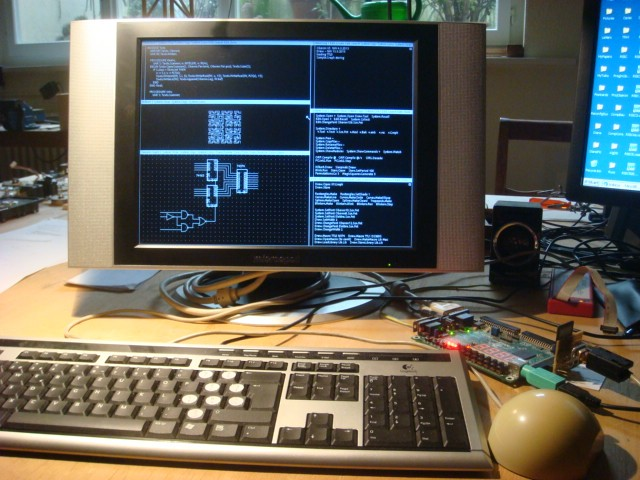
\includegraphics[width=.8\textwidth]{i/0}
\end{figure}

The decision to develop our own processor required that the compiler and linking loader chapters
had to be completely rewritten. However, it also provided the welcome chance to
improve their clarity considerably. The new processor indeed allowed to simplify and straighten out the entire compiler.

For the description of a system to be comprehensible, the key element is the notation, formalism, or
language in which it is defined. Algol 60, published 50 years ago, was proposed as a publication
language, as a formalism in which algorithms could be defined without reference to particular
computers, or to any mechanism at all. This was a great goal, but so far it was hardly achieved.
Yet, it emphasized the importance of abstraction to be achieved by the notation with a mathematically
rigorous foundation. At least, Algol was the first language based on a formally defined syntax. Algol
was the result of early recognition that programs must never be written just to feed computers,
but always to be understood and instructive to people.

In all my past work, I have tried to design a successor to Algol, that improves its rigor and at the
same time extends its applicability from numerical algorithms to software systems. From a long
sequence, starting with Algol, through Pascal, Modula, and Oberon, we have come closer to this
goal than ever before, and than any other language in existence. The key lay in a continued
struggle for sensible simplification.

The Oberon language, defined in 1988, underwent a revision in 2007, mostly discarding features
that were either duplicated or not essential. Adaptation of the system's source code to the revised
language was, besides the change of processor, the second important reason for numerous, local
changes in this text. We summarize the various deletions of features:
\begin{enumerate}
  \item The data types LONGINT, SHORTINT, and LONGREAL have been discarded, and with them the concept of type inclusion.
  \item The LOOP and EXIT statements (repetitions with multiple exit points) have been discarded.
  \item The WITH statement (regional type guard) has been discarded.
  \item The RETURN statement has been removed and is now syntactically merged with the ending of function procedure declarations.
  \item Objects declared in procedures are not accessible within their local counterparts. That is, objects must be either strictly local or global in order to be accessible.
  \item Assignments to imported variables are not permitted (read-only export).
  \item Forward procedure declarations have been discarded.
\end{enumerate}

In contrast to these removals, there is a single addition (made in 2012):
\begin{itemize}
  \item The data type BYTE has been added. Its values are integers $x$ satisfying $0 \leq x < 256$. This addition prevents the frequent abuse of the type CHAR. BYTE is mainly used for elements of arrays and records in low level modules in order to economize the use of memory.
\end{itemize}

In spite of these two reasons for changes -- one at the highest level, language, the other at the lowest, hardware -- the remainder of this book proved to be pretty stable and still valid. It has
been my desire to present the system essentially as it existed 25 years ago, without embellishments. The chapters 3 - 5 on tasking, the display and text, originally written by J. Gutknecht, have been carried over virtually unchanged. Significant changes, however, were
necessary mainly in the descriptions of device drivers for keyboard and mouse. They now use the PS-2 interface standard. The disk has been replaced by a single SD-card (flash memory) with a standard SPI interface. The net interface no longer uses RS-485, but is also based on the SPI standard. Chapters on the compiler and linker are completely new.

Mostly thanks to the regularity of RISC instruction set, the compiler size could be reduced significantly. It now measures less than 2900 lines of program and compiles itself in about 3 seconds, which is proof of its efficiency. The entire system compiles itself in less than 10 seconds.

Considered extravagant and hardly necessary only years ago, run-time checks are generated
automatically. In particular, they cover index range checks and access to NIL-pointers. Due to their
efficiency they hardly affect run-time speed, but are a great benefit to programmers.

A welcome consequence of the language and processor simplifications is the fact that all parts had been written in assembler code in 1992 -- and therefore were not included in the book -- have now been expressed in Oberon as well. Vindicating my perennial efforts to obtain a high-level
language which is powerful, flexible, and also efficient enough to express parts such as device drivers and raster operations, this was the necessary and final step to make this book comprehensive and complete.

\section*{References}
\begin{enumerate}
  \item \href{
    http://www.inf.ethz.ch/personal/wirth/Oberon/Oberon07.Report.pdf
  }{Oberon 07 Report pdf}
  \item \href{
    http://www.inf.ethz.ch/personal/wirth/FPGA-relatedWork/RISC.Arch.pdf
  }{RISC Arch pdf}
\end{enumerate}

\clearpage\section*{Acknowledgments}
I gratefully acknowledge the valuable contributions of Paul Reed. He designed the interfaces to
various devices, such as the PS-2 and SPI, including the SD-card, acting as disk store. He
suggested many improvements and simplifications. He originally decisively suggested a re-edition
of this book of 30 year ago, and was the key impetus to do all this work. My thanks go to him.
\begin{flushright}
  Niklaus Wirth, September 2013
\end{flushright}
